
\subsection*{Planes}

%%%Insert this to get the typewriter font so it looks like a real movie script
{\ttfamily
\fontdimen2\font=0.4em
\fontdimen3\font=0.2em
\fontdimen4\font=0.1em
\fontdimen7\font=0.1em
\hyphenchar\font=`\-


%%%%put a hypertarget around the opening bit of text
\hypertarget{solution_sets_for_systems_of_linear_equations_planes}{Here we want} to describe the mathematics of planes in space.
The video is summarised by the following picture:
\begin{center}
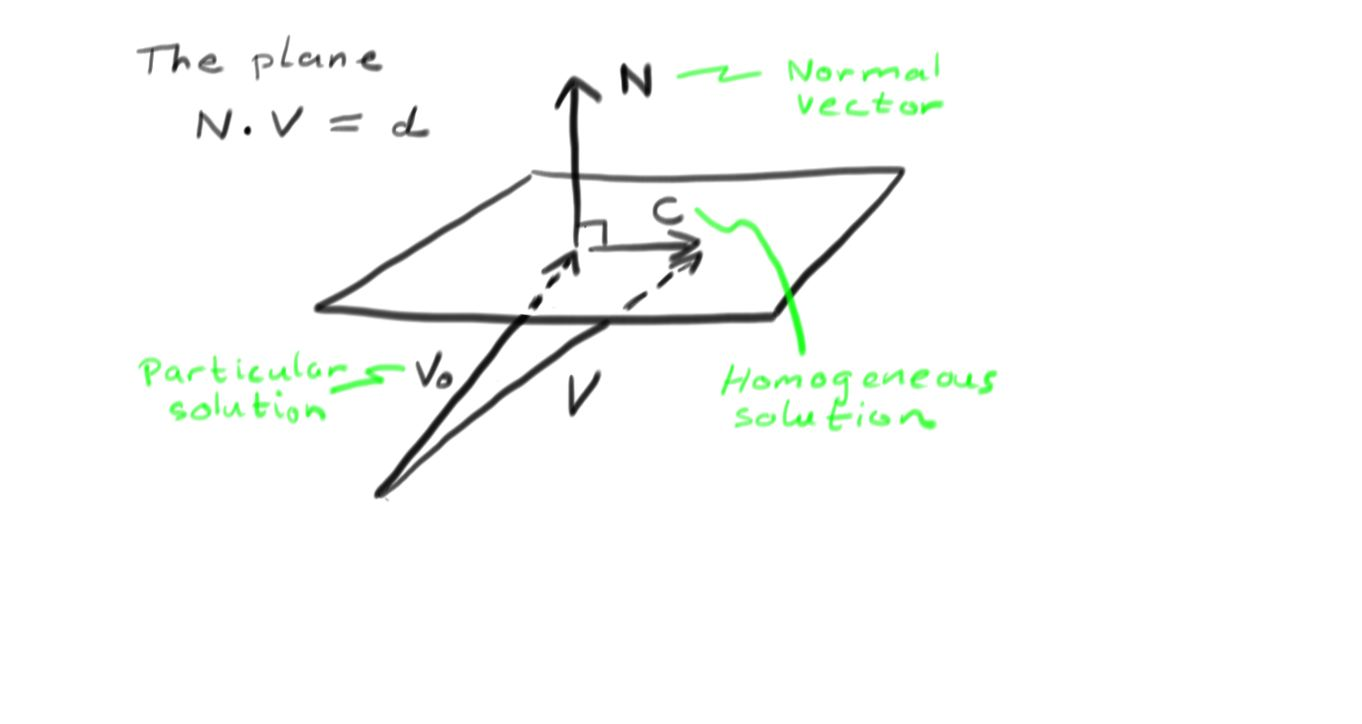
\includegraphics[scale=.2]{plane1eq.jpg}
\end{center}
A plane is often called ${\mathbb R}^2$ because it is spanned by  two coordinates, and space is called ${\mathbb R}^3$ and has three coordinates, 
usually called $(x,y,z)$. The equation for a plane is
$$
ax+by+cz=d\, .
$$
Lets simplify this by calling $V=(x,y,z)$ the vector of unknowns and $N=(a,b,c)$. Using the dot product in ${\mathbb R}^3$
we have
$$
N\dotprod V = d\, .
$$
Remember that when vectors are perpendicular their dot products vanish. {\it I.e.} $U\dotprod V = 0 \Leftrightarrow U \perp V$.
This means that if a vector $V_0$ solves our equation $N\dotprod V =d$, then so too does $V_0+C$ whenever $C$ is perpendicular to $N$.
This is because
$$N\dotprod (V_0+C) = N\dotprod V_0 + N\dotprod C = d + 0 = d\, .$$
But $C$ is ANY vector perpendicular to $N$, so all the possibilities for $C$ span a plane whose normal vector is $N$. Hence we have shown that 
solutions to the equation $ax+by+cz=0$ are a plane with normal vector $N=(a,b,c)$.



%%%%don't forget to close the bracket so the stuff after your file doesn't look like a movie!
}

%\newpage
